\documentclass[10pt,twocolumn,letterpaper]{article}

\usepackage{cvpr}
\usepackage{times}
\usepackage{epsfig}
\usepackage{graphicx}
\usepackage{amsmath}
\usepackage{amssymb}
\usepackage{listings}
\usepackage{subcaption}

% Include other packages here, before hyperref.

% If you comment hyperref and then uncomment it, you should delete
% egpaper.aux before re-running latex.  (Or just hit 'q' on the first latex
% run, let it finish, and you should be clear).
\usepackage[breaklinks=true,bookmarks=false,hidelinks]{hyperref}

\cvprfinalcopy % *** Uncomment this line for the final submission

\def\cvprPaperID{****} % *** Enter the CVPR Paper ID here
\def\httilde{\mbox{\tt\raisebox{-.5ex}{\symbol{126}}}}

% Pages are numbered in submission mode, and unnumbered in camera-ready
%\ifcvprfinal\pagestyle{empty}\fi
\setcounter{page}{1}
\begin{document}

%%%%%%%%% TITLE
\title{ Semantic Segmentation for Unnamed Surface Vessle Navigation}

\author{Martin Cote\\
ME780 Perception For Autonomous Driving\\
University of Waterloo\\
{\tt\small m4cote@uwaterloo.ca}
}

\maketitle
%\thispagestyle{empty}

%%%%%%%%% ABSTRACT
\begin{abstract}
 Semantic Segmentation is the task of making pixel wise classification of an image. It is currently a popular area of research in the deep learning community, and has many potential applications in the real world. For this project, I will be exploring it's use in a marine environment, where it could be used for remote surveys in storm water ponds, or even at open-seas for detecting land or other obstacles. The first step was to collect a dataset to be used with a convolution neural network. This dataset was collected using an unnamed surface vehicle, and was labeled by hand as either "water" or "land". Dataset augmentation techniques were applied to effectively increase the total number of training and testing example. Once the data was collected and labeled, it was used as input into a convolution neural network based on the popular SegNet architecture developed by Vijay Badrinarayanan et al.~\cite{DBLP:journals/corr/BadrinarayananK15} It was shown this particular implementation of SegNet performed with a very high level of accuracy and converged fairly quickly. It was suggested this was due to the predictable nature of the dataset and low number of potential classes. The resulting inference time of the implemented network is such that it could be used real time on an autonomous surface vehicle in a research environment, but would likely require further optimization to be used in an industrial environment. Similarly the GPU memory requirements are reasonable to have on board an autonomous vehicle, but were unfortunately greater than the hardware setup used for this project. The next steps for this project would be to collect data in new and unique environments, and develop a control system to make use of the segmentation data. All related code and dataset are available on my GitHub page, https://github.com/majcote/ME780-project
\end{abstract}


%%%%%%%%% INTRODUCTION
%This section introduces your problem, and the overall
%plan for approaching your problem.

\section{Introduction}
For my final project in ME780, I plan to address the task of semantic segmentation
for the use of autonomous navigation of an unmanned surface vessel (USV). I will be 
doing pixel wise classifications of images from a camera mounted to the USV. For the
purpose of this project, I will only require 2 classes, water and other. This task
has several useful applications for the marine industry, such as remote surveys and open seas navigation. Classifications of open water is a part of the full stack required to do safe marine autonomy,
similar to classifying drivable roads in autonomous driving applications.

This project is largely motivated by future projects from my place of employment.
I work for Clearpath robotics, in the research solutions department. We build 
custom robots for the use in robotics research. However we are now looking
towards the remote survey industry, that is, using robotics to remotely survey
environments that are too dirty, dull or dangerous for humans. One such task is 
remote marine surveys, wherein a USV is used to collect data from a body of water
while the operator can stay safely on shore. Clearly a very important part of this
task is to determine if the USV has clear water ahead of it, or it will risk 
running aground.

\begin{figure*}[h]	
\begin{center}
  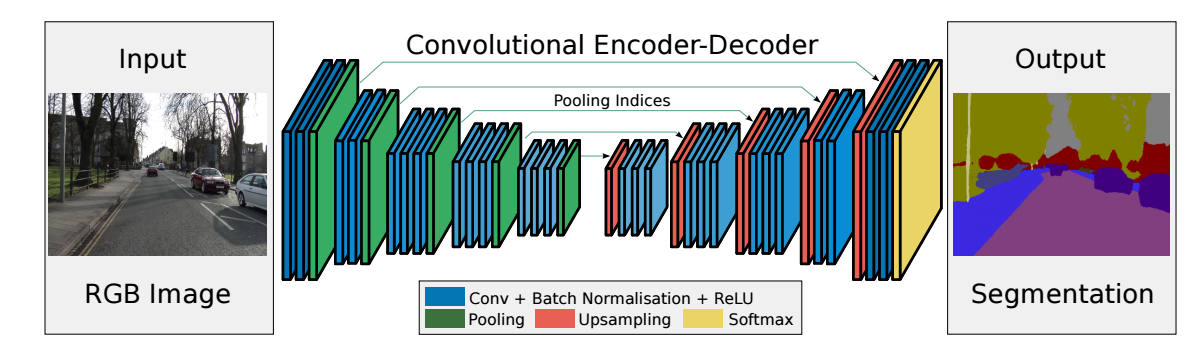
\includegraphics[width=1.0\linewidth]{Segnet_architecture.png}
\end{center}
   \caption{The encoder-decoder network architurecture used for SegNet, and similary used for this porject~\cite{DBLP:journals/corr/BadrinarayananK15}}
\label{fig:Segnet_architecture}
\end{figure*}

\begin{figure}[b]	
\begin{center}
  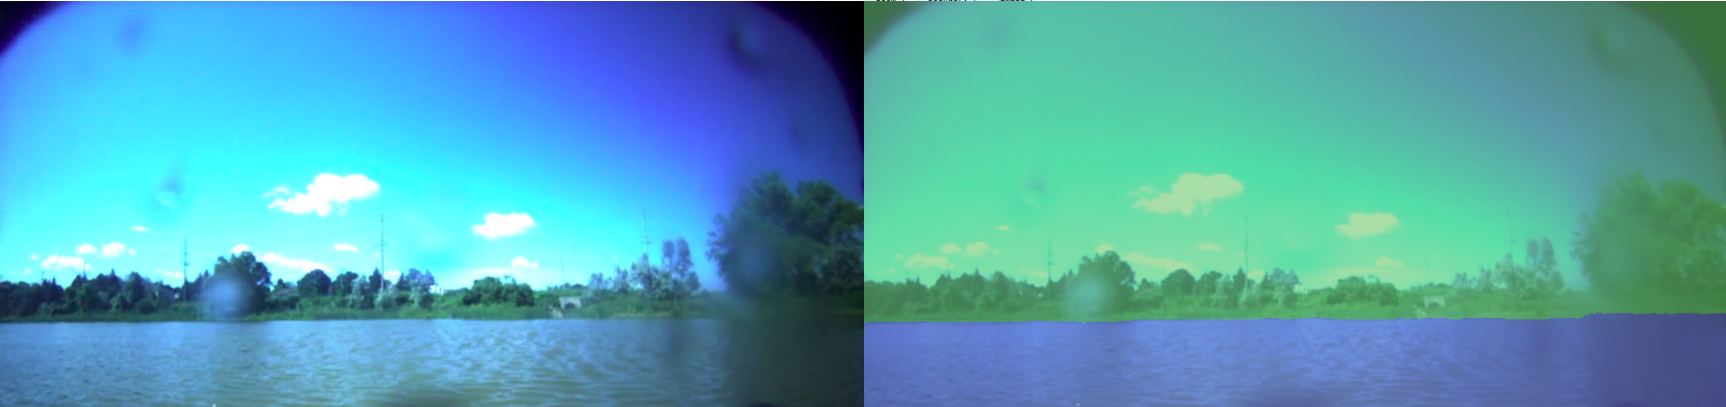
\includegraphics[width=1.0\linewidth]{segmenttool.png}
\end{center}
   \caption{Screen shot of annotation tool used, where the blue mask corresponds to the water class, and green is other}
\label{fig:tool}
\end{figure}

I therefore propose to use concepts discussed in ME780, Perception For Autonomous Driving,
and adapt them for use on a marine vehicle in bodies of water. My goal for this project
is to implement a convolution neural network to make pixel wise classification of an image
from an onboard camera as either "water" or "other". To the best of my knowledge, there is no
dataset publicly available to be used for this task, therefore a large portion of my project will be 
dedicated to collecting and preparing data to be used for training, testing and evaluation of my network. 
My network will be evaluated on both run time and accuracy. I expect this
implementation to be able to do classifications with sufficient level of accuracy, however
minimizing the runtime to be able to do live classifications may be more challenging.

%-------------------------------------------------------------------------
%%%%%%%%% Background/Related Work
%This section discusses relevant literature
%for your project

\section{Related work}
The task of semantic segmentation is currently a popular area of research in the deep learning community, 
it involves involves classification at a per pixel level, this results in a better understanding of the scene by providing not only information on the object, but where the object is located. ~\cite{DBLP:journals/corr/Thoma16a}. This has many useful application such as detecting road signs, drivable road and obstacle avoidance  ~\cite{4220659} ~\cite{BMVC2015_109} in autonomous driving. 

\subsection{SegNet}

I will applying SegNet's architecture ~\cite{DBLP:journals/corr/BadrinarayananK15} for my own task of semantic segmentation. Segnet is a deep convolution neural network which uses an encoder-decoder architecture for segmentation segmentation, developed by the team from the Computer Vision and Robotics Group at the University of Cambridge. SegNet
is novel in it's use of the encoder-decoder network architecture as shown in figure ~\ref{fig:Segnet_architecture}. The first 13 layers of this network make up the encoder portion, which is in fact
the first 13 layers of the VGG16 Network ~\cite{DBLP:journals/corr/SimonyanZ14a}. The encoder layer consists of a convolution layer, followed by a batch-normalization layer ~\cite{DBLP:journals/corr/IoffeS15}, a ReLU activation function and finally a max pooling layer which results in an output which half the size as it's input~\cite{DBLP:journals/corr/BadrinarayananK15}. The decoding layers upsamples using max-pooling with
the same indices that were used in the encoding layers, followed by another set of convolution layer, batch normalization, and ReLU activation. Due to the up sampling layers, the output of the decoder layers are the same size as the input image size to the network, this output is then passed through a softmax regression layer to
make pixel wise perditions. SegNet was chosen for this project due to it's competitive performance in other 
segmentation data sets, as well as it's smaller set of parameters which makes for quicker training.

\subsection{Fancy PCA}
Fancy PCA is a dataset augmentation technique proposed by Alex Krizhevsky et al.~\cite{NIPS2012_4824}. It can be used to greatly increase the number of images in a dataset, it involves altering the intensities of each RGB pixel value slightly throughout the full training set. Each RGB pixel value for the entire training set is concatenated and the covariance matrix is calculated. From the covariance matrix, the eigenvectors and eigenvalues are also found, the highest value eigenvectors is the principle components ~\cite{FancyPCA}. Multiples of the found principle components, with magnitudes proportional to the corresponding eigenvalues times a random variable from a Gaussian distribution, are added to every pixel value ~\cite{NIPS2012_4824}.  Alex Krizhevsky et al. suggests that object identity is invariant to changes in the intensity and color of the illumination, thus each new image that's created contains new valuable information for training neural networks.

%-------------------------------------------------------------------------
%%%%%%%%% Technical approach
%Describe the methods you intend to apply to
%solve the given problem.

\section{Technical Approach}
\subsection{Data Collection}
As previously mentioned, there is no publicly available dataset for use in a marine
environment to the best of my knowledge, therefore the first part of this project
will be collecting such a dataset. To do so, I've used Clearpath Robotics's
Heron platform with an onboard Point Grey Chameleon camera as shown in figure ~\ref{fig:heron}

\begin{figure}[h]	
\begin{center}
  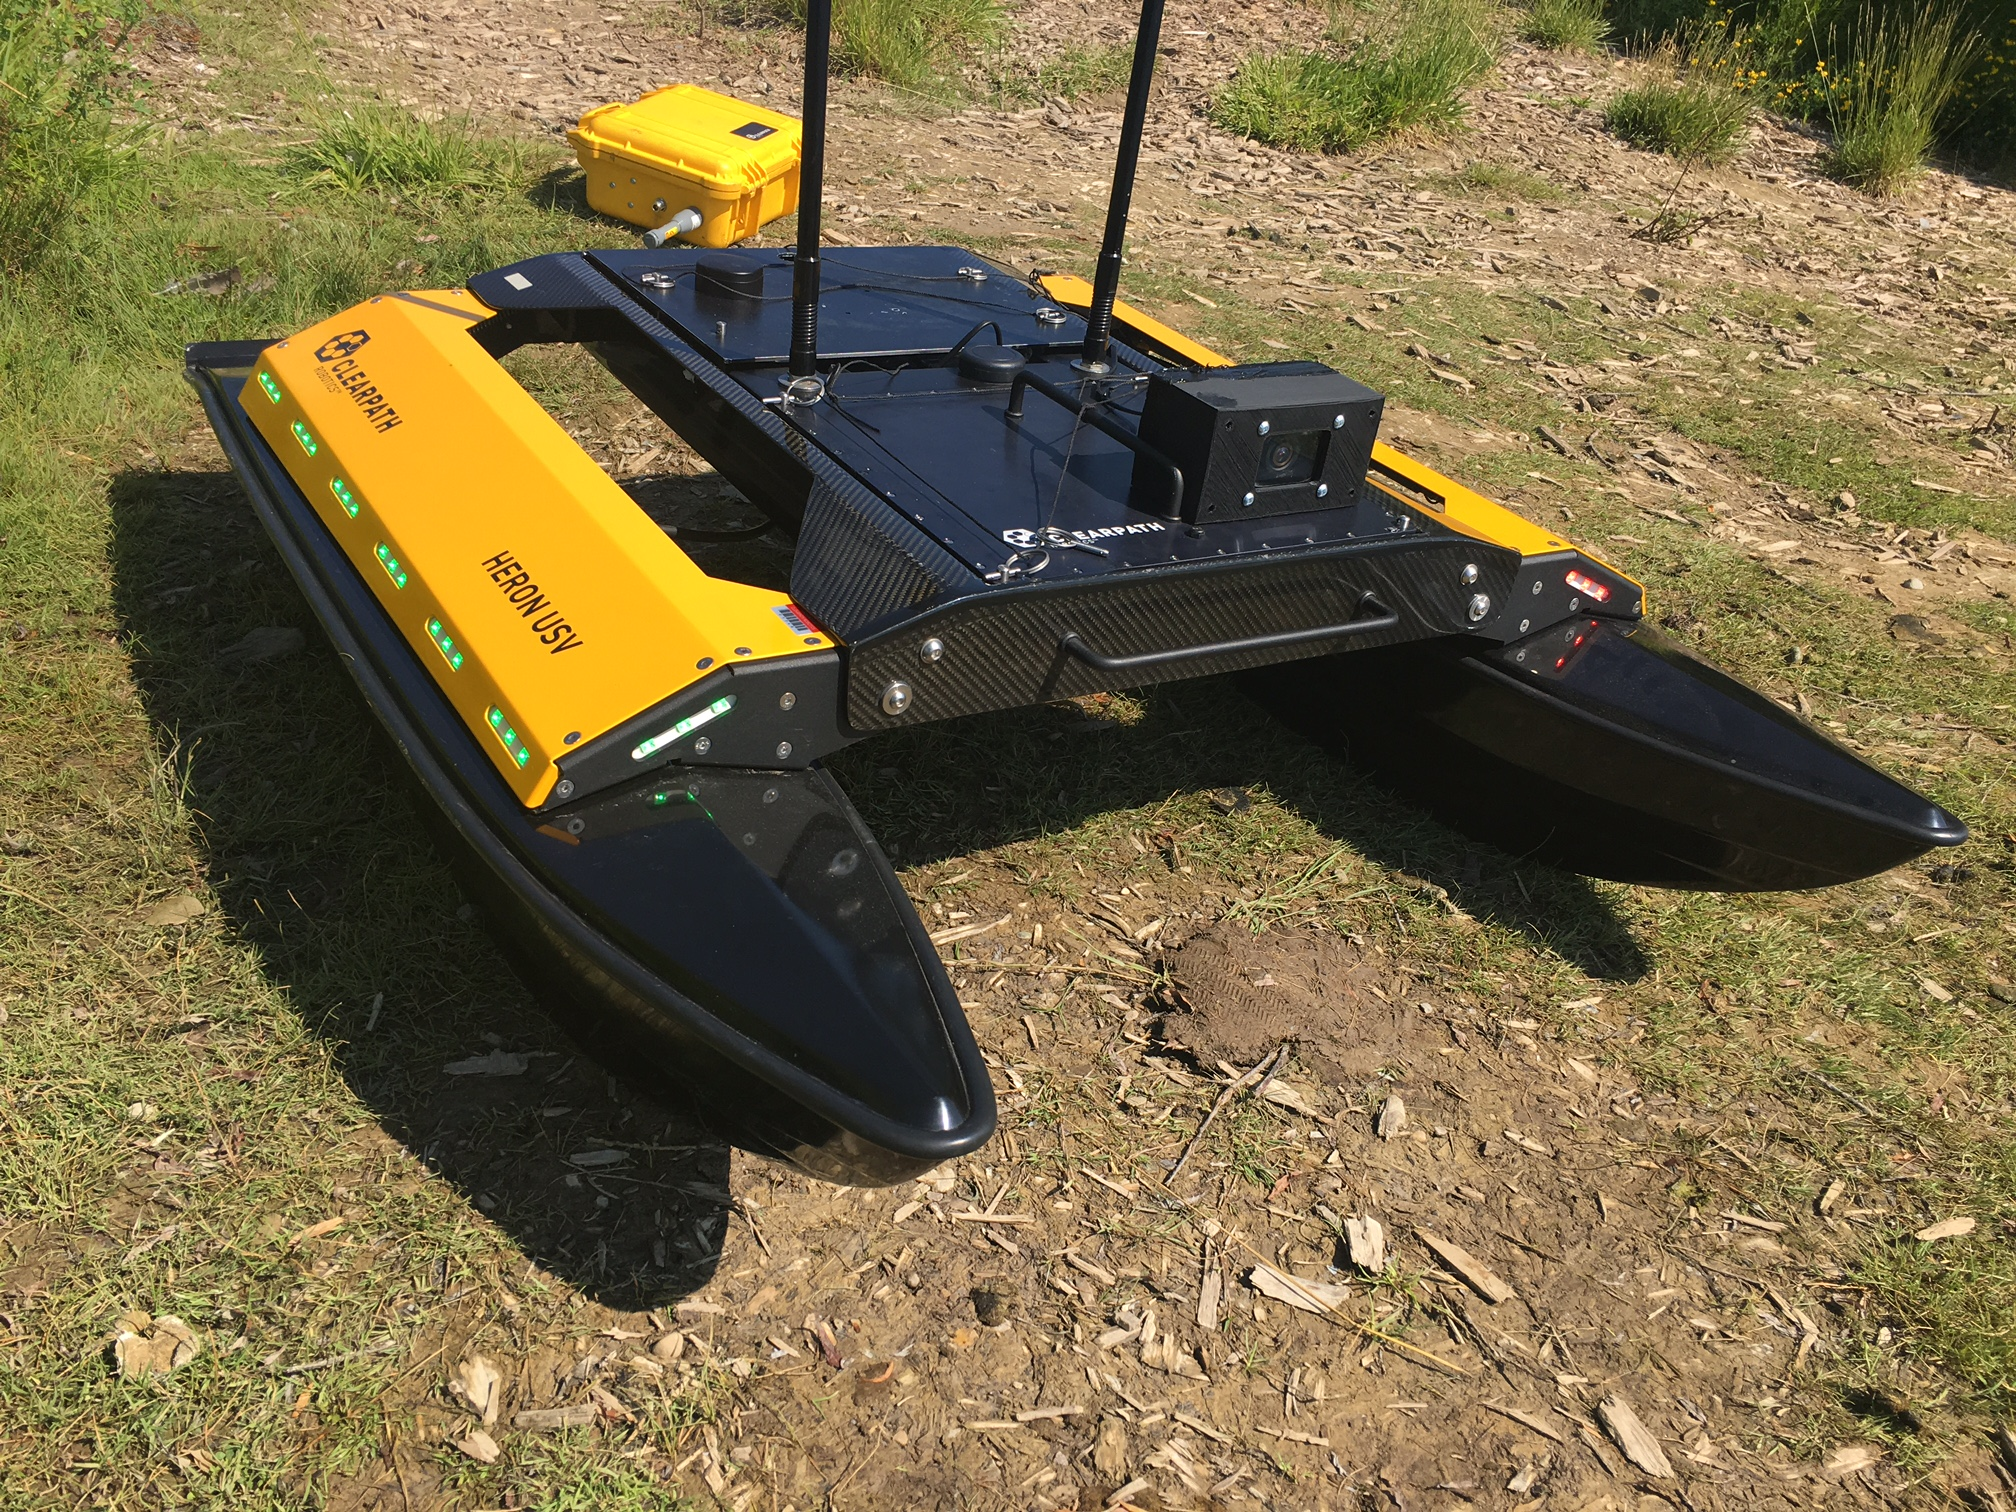
\includegraphics[width=1.0\linewidth]{heron.JPG}
\end{center}
   \caption{Clearpath Robotics's Heron with mounted Camera for marine data collection}
\label{fig:heron}
\end{figure}


The data was collected in a ROS bag, along with other important ROS topics that may be used
for future work. The ROS topic \verb|camera\image_color|, was extracted and 
converted into a mp4 file using the \verb|bag_tools| ROS package ~\cite{bagtools}. PNG images
were then be extracted from the mp4 files at a rate of once every 2 seconds.


\subsection{Data Preparations}
Once the images have been collected, they must now be prepared for use with the neural network.
The images must be labeled at a pixel level as either "water" or "other". To simplify classification,
the images will be cropped to remove static portions of the images that do not need to be classified,
such as the outline of the boat itself, and the inside of the camera enclosure.

The images will be labeled using the \verb|js-segment-annotator| tool that was developed for related
segmentations work ~\cite{tangseng2017looking}. The output is an PNG image with different RGB values for each class (the difference is subtle, and not visible to the human eye). These images are then to be converted to gray scale, and the specific RGB value corresponding to each label is mapped to a corresponding single channel gray intensity.



\subsection{Dataset Augmentation}
Two techniques were employed to effectively increase the number of training examples. The first is simply mirroring all images horizontally. This can be done quite easily through \verb|imagemagick| command line tools.

The second technique to be implemented is the Fancy PCA technique presented in related work. This was implemented through an IPython notebook. The code which was used is be based on a tutorial written by Deshana Desai~\cite{FancyPCA}, and is now committed to my personal Github

\subsection{Segmentation}
Once the collected data is prepared, it is to be used with an implementation of SegNet~\cite{DBLP:journals/corr/BadrinarayananK15}. The network architecture should remain fairly unchanged, however slight changes will be required to satisfy my GPU limitation (GTX770), and change the number of classes. SegNet will be run using a modified version of Caffe~\cite{jia2014caffe} intended for use with SegNet and uses cuDNN5\cite{caffe-segnet-cudnn5}.

%-------------------------------------------------------------------------
%%%%%%%%% Experiments
%This section begins with what kind of experiments
%you’re doing, what kind of dataset(s) you’re using, and what is the
%way you measure or evaluate your results. It then shows in details the
%results of your experiments. By details, we mean both quantitative
%evaluations (show numbers, figures, tables, etc) as well as qualitative
%results (show images, example results, etc).
\begin{figure*}[hpt]
\begin{center}
	
	\begin{subfigure}{0.3\textwidth}
  		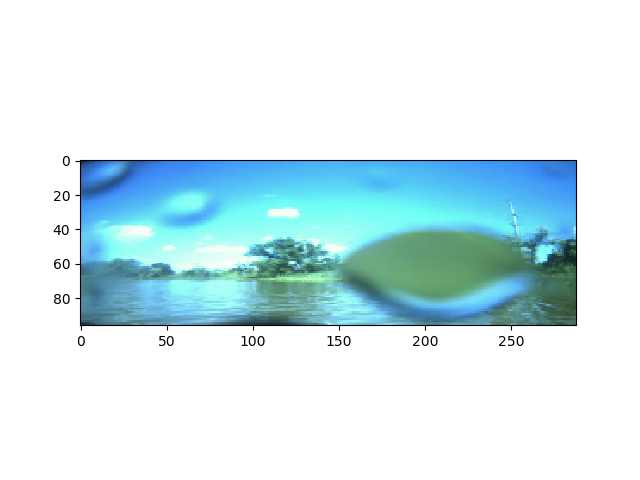
\includegraphics[width=\linewidth, trim={1.25cm 1.5cm 1.5cm 1.25cm},clip]{image1.png}
  		\caption{Image}
  	  \end{subfigure}
  	  \hfill
  	  \begin{subfigure}{0.3\textwidth}
  		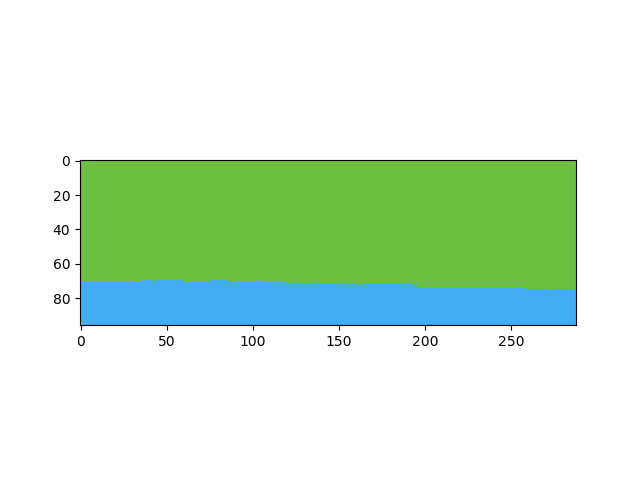
\includegraphics[width=\linewidth,trim={1.25cm 1.5cm 1.5cm 1.25cm},clip]{gt1.png}
  		\caption{Ground Truth}
  	\end{subfigure}
  		\hfill
  	\begin{subfigure}{0.3\textwidth}
  		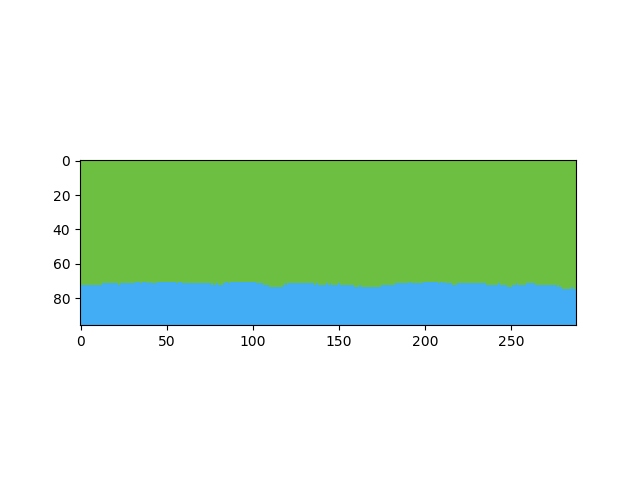
\includegraphics[width=\linewidth,trim={1.25cm 1.5cm 1.5cm 1.25cm},clip]{perdiction1.png}
  		\caption{Perdiciton}
  \end{subfigure}
  
  	\begin{subfigure}{0.3\textwidth}
  		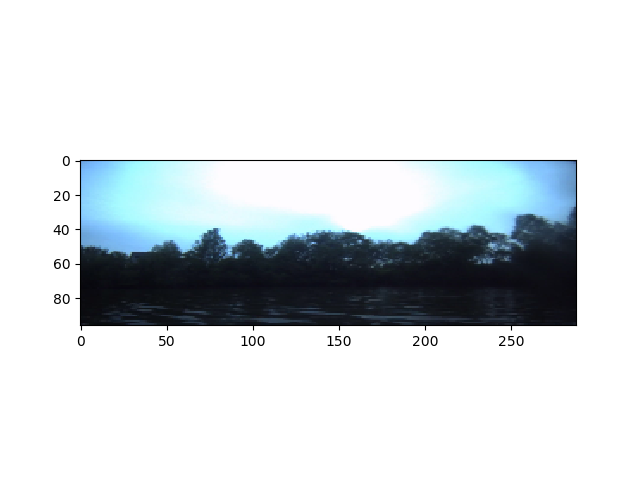
\includegraphics[width=\linewidth, trim={1.25cm 1.5cm 1.5cm 1.25cm},clip]{image2.png}
  		\caption{Image}
  	  \end{subfigure}
  	  \hfill
  	  \begin{subfigure}{0.3\textwidth}
  		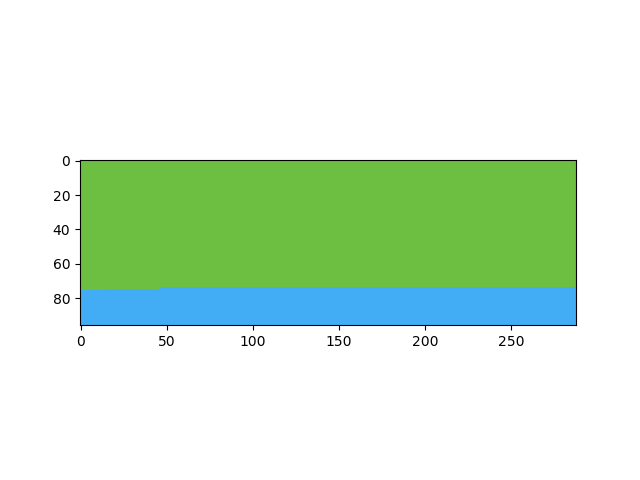
\includegraphics[width=\linewidth,trim={1.25cm 1.5cm 1.5cm 1.25cm},clip]{gt2.png}
  		\caption{Ground Truth}
  	\end{subfigure}
  		\hfill
  	\begin{subfigure}{0.3\textwidth}
  		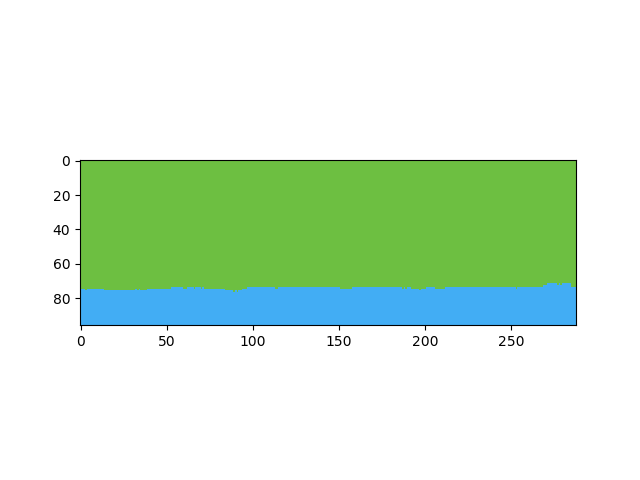
\includegraphics[width=\linewidth,trim={1.25cm 1.5cm 1.5cm 1.25cm},clip]{perdiction2.png}
  		\caption{Perdiciton}
  \end{subfigure}
  
  
  	\begin{subfigure}{0.3\textwidth}
  		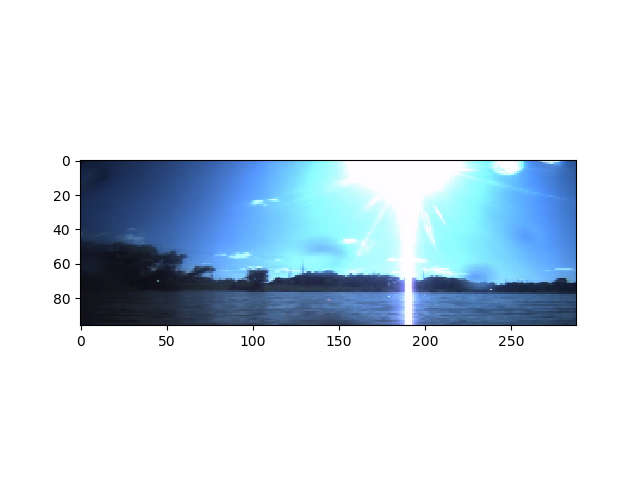
\includegraphics[width=\linewidth, trim={1.25cm 1.5cm 1.5cm 1.25cm},clip]{image4.png}
  		\caption{Image}
  	  \end{subfigure}
  	  \hfill
  	  \begin{subfigure}{0.3\textwidth}
  		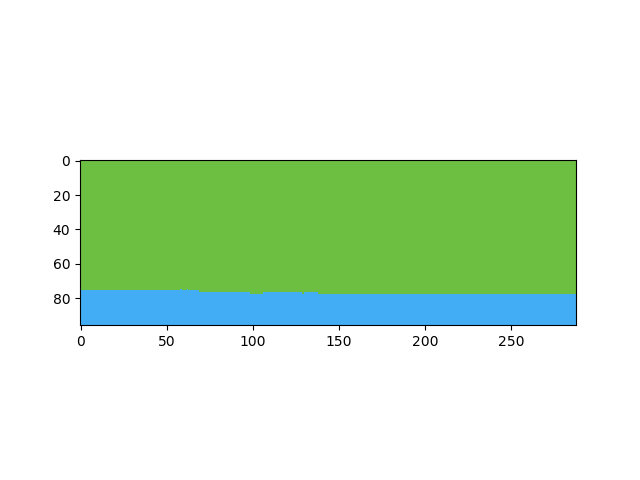
\includegraphics[width=\linewidth,trim={1.25cm 1.5cm 1.5cm 1.25cm},clip]{gt4.png}
  		\caption{Ground Truth}
  	\end{subfigure}
  		\hfill
  	\begin{subfigure}{0.3\textwidth}
  		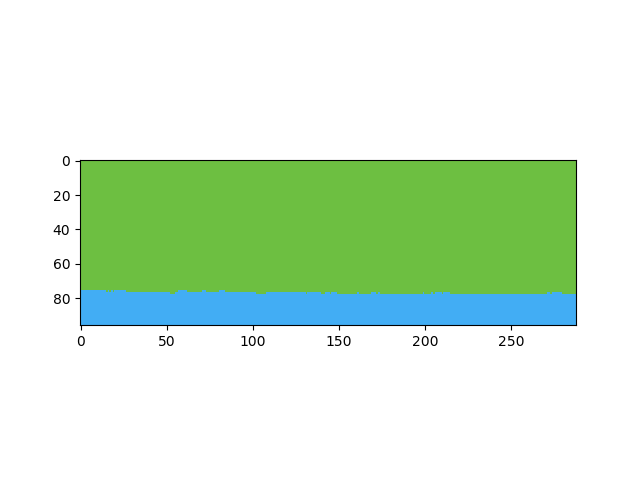
\includegraphics[width=\linewidth,trim={1.25cm 1.5cm 1.5cm 1.25cm},clip]{perdiction4.png}
  		\caption{Perdiciton}
  \end{subfigure}
  
    	\begin{subfigure}{0.3\textwidth}
  		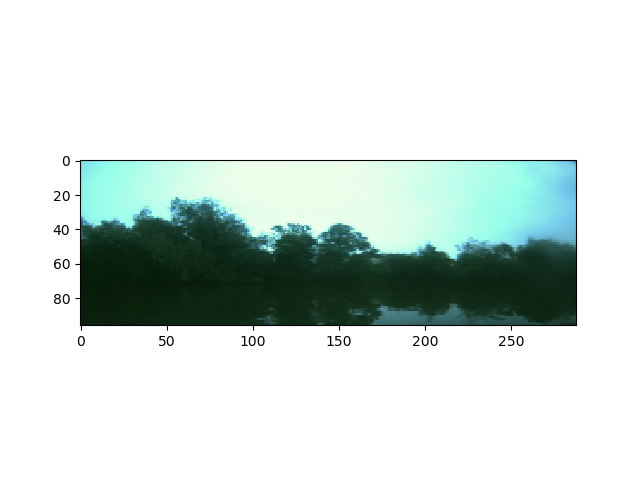
\includegraphics[width=\linewidth, trim={1.25cm 1.5cm 1.5cm 1.25cm},clip]{image5.png}
  		\caption{Image}
  	  \end{subfigure}
  	  \hfill
  	  \begin{subfigure}{0.3\textwidth}
  		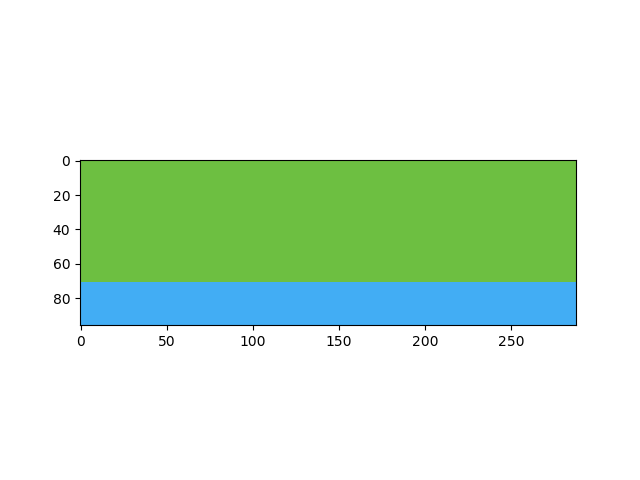
\includegraphics[width=\linewidth,trim={1.25cm 1.5cm 1.5cm 1.25cm},clip]{gt5.png}
  		\caption{Ground Truth}
  	\end{subfigure}
  		\hfill
  	\begin{subfigure}{0.3\textwidth}
  		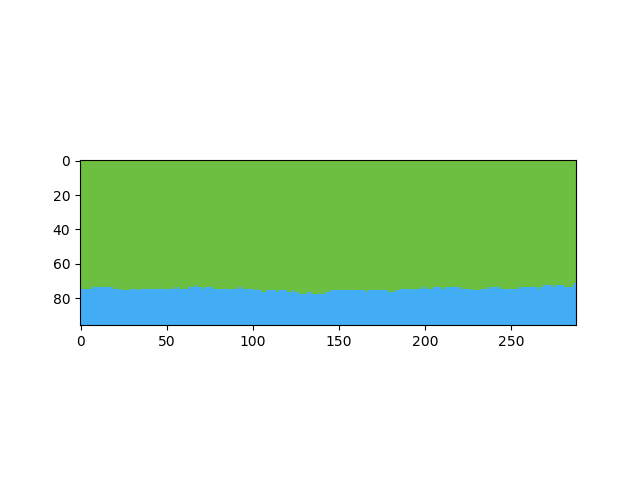
\includegraphics[width=\linewidth,trim={1.25cm 1.5cm 1.5cm 1.25cm},clip]{perdiction5.png}
  		\caption{Perdiciton}
  \end{subfigure}
  
  
 
\end{center}
   \caption{Examples of testing images used, as well as the associated ground truth, and prediction output}
\label{fig:prediction_results}
\end{figure*}
\section{Experiments}

\subsection{Dataset preparation}
The result from 3 data collections at ponds in the Waterloo region was 185 fairly unique images. Cropping the images was done using \verb|imagemagick| command line tools. Labeling the images was a very time consuming task, however the utility that was used was fairly straight forward to configure and use. Figure ~\ref{fig:tool} shows the classification that was done by hand using this utility. All pixels were labeled as either "water" or "other". Once labeled, the images were mirrored resulting in 370 images, the annotated image were also mirrored at this time. Finally the Fancy PCA algorithm was applied to the entire set of images (Ipython code is available on my Github), resulting in a total of 740 images. The annotated images did not need modification, and were just paired with their Fancy PCA counterparts. A Dropbox link to this dataset is available on Github for anyone else who may also want to do similar work. The full dataset was randomly split to 60\% training set, 20\% test set and 20\% evaluation set.


\begin{figure}[b]	
\begin{center}

	\begin{subfigure}{0.5\textwidth}
  	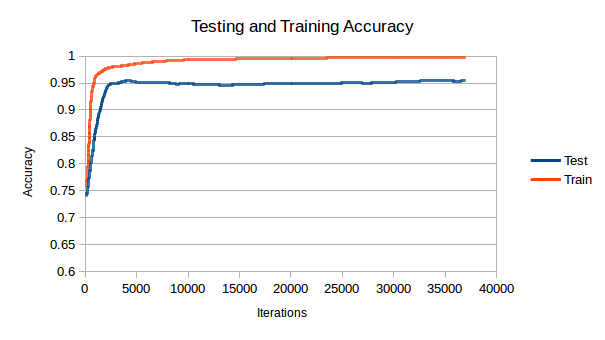
\includegraphics[width=1.0\linewidth]{Accuracy_chart.png}
  	\end{subfigure}
   
   \begin{subfigure}{0.3\textwidth}
   \begin{tabular}{| c | c | c | }
   \hline
	Itreration	&	Test	&	Train\\ 
 	\hline 
	100	&	0.739507	&	0.758109\\ 
 	\hline 
	1000	&	0.860782	&	0.96172\\ 
 	\hline 
	5000	&	0.951749	&	0.985958\\ 
 	\hline 
	10000	&	0.949844	&	0.992914\\ 
 	\hline 
	20000	&	0.949318	&	0.995751\\ 
 	\hline 
	25000	&	0.950198	&	0.996827\\ 
 	\hline 
	30000	&	0.9518	&	0.997147\\ 
 	\hline 
	35000	&	0.954353	&	0.997615\\
	\hline
	\end{tabular}   
	\end{subfigure}
	
\end{center}
\caption{Testing and training accuracy over interations}
\label{fig:accuracy}
\end{figure}

\subsection{Segmentation}
As previously mentioned, the SegNet network architecture was used. The input images into SegNet required rescaling due to GPU limitation on my home desktop. Initial weights from VGC16 were used to initialize the network. After training the network for close to 37000 iterations, a training accuracy of 99\% was achieved. Weights were snapshotted at every 1000 iterations, and
performance was tested on the test set with the saved weights. As you can see from figure ~\ref{fig:accuracy}, the network very quickly converged to near 95\% accuracy even on the test set.These results may suggest there is not much over fitting to the training set as the performance on the test set did not decrease as the number of iterations increased. However it should be noted, it's also possible my collected data set was similar enough across both the training and test set that my test set was not in fact a good test on the networks generalization error.

Figure~\ref{fig:prediction_results} shows some sample results, the first image is the input image, the second is the ground truth which was labeled by hand using the annotation tool mentioned above, and the third image is the output of neural network.
I chose too highlight these instances because they have features that are out of the norm. The first set of examples shows water droplets on the camera enclosure, as you can see from the prediction results, the network was nevertheless able to determine the class behind the water droplet. The second set of images, shows an instance of relatively low light, this particular image was near the end of the day and it's difficult to determine the separation between the water line and shore, though the prediction was still able to separate water and land . The third set of images shows the opposite, this was a mid day shot with much more lighting, so much so there is glare across the image, however it's clear this did not effect the prediction. The final set of images shows another instance where it's difficult to separate the shore and water, furthermore, this image has a green tint which is unlike the others.

\begin{table*}[pt]
\begin{center}
\resizebox{\textwidth}{!}{
\begin{tabular}{| c | c | c | c | c |}
\hline
  Forward Pass(ms) & Backwards Pass(ms) & Forward and Backwards pass(ms)& GPU Training memory (MiB) & GPU Infrence Memory (Mib) \\
  \hline
  1348.78 & 1298.7 & 2647.5 & 1049 & 1908 \\
  \hline
\end{tabular}}
 \caption{Forward and backwards times measured using the caffe time command over 10 iterations with a batch size of 1, and memory usage found using the nvidia-smi command  }
 \end{center}
\label{tab:time}
\end{table*}

One of the most obvious similarities is in fact the ground truth. I believe this is one of the main reasons the network performed so well. Due to the mounting location of the camera and it's field of view, the water line is largely in the same area across most iamges, with the "water" class below and the "other" class above. This semantic information that "other" is always above "water" at a certain point, has no doubt contributed to the networks confidence that despite in some images, both the sky and water are blue for example, it knows there is a point where the labels switch quite abruptly. It is this predictability in each label's general location, and size, which I believe contributed to the high accuracy predictions.

In comparison, the original implementation of SegNet was only able to achieve 90\%+ accuracy in a few classes, despite it being one of the most accurate networks for semantic segmentation ~\cite{DBLP:journals/corr/BadrinarayananK15}. I believe the difference in performance between it's use in object and road classification and my collected data is the increased number of classes and more randomness in it's input images. These use cases aren't able to rely on the very clear water / other borderline as my network was. To reinforce this argument, it's interesting to note that according to the analysis in the paper which presented SegNet~\cite{DBLP:journals/corr/BadrinarayananK15}, it seems most networks are able to classify roads with relative ease. I believe this is due to the same reason that my network performed so well, that is predictable location and relative size with respect to the position of the camera.

As the end goal would be to run this neural network real time on marine vehicles, the memory usage and inference time is very important. The forward pass time and memory requirements can be found in table 1. Though the inference would be too slow for an autonomous land vehicle, marine vehicles often have more time to react. It would certainly be preferable to bring this time down closer to what is expected for land vehicles, however for a research setting, I feel this is acceptable to use on board. Unfortunately the memory requirements are greater than what's available on Clearpath robotics Heron platform by default, however these requirements are not unrealistic for an autonomous vehicle. 


%-------------------------------------------------------------------------
\section{Future Work}
There are two paths that I would like to pursue with this project. The first would be to collect more data in more unusual environments and different angles. I feel confident this implementation would be able to navigate the small ponds and lakes within the Waterloo region, however the next step would be to collect data in larger bodies of water, ideally even in the ocean. I would like to try to simulate environments where the shore line would not necessarily be so similar between images, or cases where there isn't a shore in sight, but simply water and sky. There is a very practical real world use for this type of classification. At the present time, large ships, such as cargo ship or cruise ship, always have a crew member surveying the horizon for anything that isn't water, as you can imagine this can be a very dull task. There is indeed a demand for technology that could autonomously survey the horizon and notify the crew of any abnormalities.

The other path to pursue would be to run this network on an autonomous surface vehicle, and study how the segmentation information can be used to navigate safely and autonomously. Control systems could be developed to navigate based on the amount of shore that is visible, and where the shore line is relative to the robot position. As mentioned previously, this could have many applications in the remote marine survey industry.

Unfortunately at this time I am blocked on pursuing either of these paths. I do not feel I'll be able to collect data from sufficiently different environment without traveling outside of the Waterloo region, or further, and I'm limited by hardware to run my implementation of SegNet on board a USV.

\section{Conclusion}
Semantic segmentation is currently a popular area of research in the deep learning community, I have yet to seen it implemented in a marine environment, despite the many practical real world applications. In this project, I collected data using a Unnamed surface vehicles and had to work through the many intricacies in preparing this data for use in a convolution neural network. Due to the limited dataset, I also explored and implemented dataset augmentation techniques to effectively increase the number of input images to be used for training and testing. Once the data was collected, it needed to be labeled for use for supervised training which was a very laborious task. This labeled data was then used as input into an implementation of the popular semantic segmentation network, SegNet~\cite{DBLP:journals/corr/BadrinarayananK15}. It was shown that this network was able to converge relatively quickly and make predictions with high accuracy. It was suggested this was due to the predictability in the relative position and size of each class with respect to the camera position on the vehicle. The ultimate goal of this project is to run this network on board an unmanned surface vehicle, it was shown that though there is room for improvement with regards to inference time, this network could be run on board (with the correct hardware) at a level which I believe would allow for autonomous operations.
On a personal level, I'd just like to mention this project, and course as a whole, has been a great learning experience! Coming from a non computer science background, with no previous machine learning experience, it has been a pleasure to be able to work through all aspects of deep learning, form collecting and labeling a data set, to running my own convolution neural network at home and accurately make prediction on said data set. It all felt very rewarding!


{\small
\bibliographystyle{ieee}
\bibliography{egbib}
}

\end{document}
